\subsection{Quelle longueur d'onde du laser ?}

La structure interne de l'atome est modélisée par un système à deux niveaux, et la polarisabilité de l'atome est décrite par le modèle classique de Lorentz {\color{red}[9902072]}. En utilisant les notations suivantes : $\omega_0$ pour la fréquence propre entre ces deux niveaux et $\omega$ pour la fréquence du faisceau laser, lorsque le désaccord est négligeable par rapport à la fréquence du laser ($|\omega - \omega_0| \ll \omega_0$), le taux d'amortissement classique est donné par :

\begin{eqnarray}\label{eq:amort.classique}
	\Gamma ( \omega )  = \frac{ e^2 }{6 \pi \epsilon_0 m_e c^3 } \omega^2 
\end{eqnarray}

Cela conduit à l'expression suivante :

\begin{eqnarray}
	\hbar \Gamma_{sc} = \frac{\Gamma_0}{ \omega - \omega_0 }U_{dip}
\end{eqnarray}

où $\Gamma_0 \equiv \Gamma ( \omega_0 )$.

À partir de cette dernière équation, on peut établir une relation entre la longueur d'onde du laser $\lambda$, le potentiel dipolaire $U_{dip}$ et le taux de photons diffusés $\Gamma_{sc}$. Si l'on impose les conditions suivantes :

\begin{itemize}
	\item Le potentiel dipolaire $U_{dip}$ doit être supérieur à $U_{dip , \text{min}}$.
	\item $\Gamma_{sc}$ pour une valeur de $U_{dip}$ doit être inférieur à $\Gamma_{sc , \text{max}}$.
\end{itemize}

On obtient alors la longueur d'onde maximale $\lambda_{\text{max}}$ que le laser peut avoir :

\begin{eqnarray}
	\lambda  =  \frac { 1 }{ \frac{\Gamma_0 }{\Gamma_{sc} }\frac{U_{dip}}{ h c } + \frac{ 1 }{\lambda_0}} \leq  \frac { 1 }{ \frac{\Gamma_0  }{\Gamma_{sc , \text{max}} }\frac{U_{dip , \text{min}}}{ h c } + \frac{ 1 }{\lambda_0}} = \lambda_{\text{max}}
\end{eqnarray}

Nous prenons $U_{dip , 0 , \text{min}}/k_B = 1 ~\mu K$ comme valeur minimale du potentiel dipolaire, et le taux de diffusion des photons pour $U_{dip , \text{min}} = U_{dip , 0 , \text{min}}/2 = 500 ~nK \times k_B$ est $\Gamma_{sc , \text{max}} = 1~s^{-1}$. Nous nous plaçons autour de la transition $D_2$ du rubidium 87, c'est-à-dire à une {\color{red}longueur d'onde propre $\lambda_0 = 780 ~\text{nm}$} {\color{red} Nous obtenons ainsi $\lambda_{\text{max}} = 779,228 ~\text{nm}$, ce qui correspond à un décalage de moins de $1~\text{nm}$.}\\

\subsection{Quelle Puissance  du laser ?}

Le potentiel dipolaire s'exprime par l'équation suivante :

\begin{eqnarray}\label{eq:potentiel.dip.simple.classique}
	U_{dip}(\vec{r}) = \frac{3 \pi c^2}{2 \omega_0^3} \frac{\Gamma_0}{\omega - \omega_0} I(\vec{r})
\end{eqnarray}

où $I(\vec{r})$ est l'intensité du champ laser. On modélise cette intensité par l'intensité d'un faisceau gaussien :

\begin{eqnarray}
	I(\vec{r}) = \frac{2P}{\pi w^2(z)} e^{-\frac{2x^2}{w^2(z)}}
\end{eqnarray}

avec $P$ la puissance du faisceau laser, $w(z)$ le diamètre du faisceau laser à la position $z$, $w_0$ la waist, et $z_R = \pi w_0^2/\lambda$ la longueur de Rayleigh du laser. Étant donné que les atomes se trouvent proches du point focal du faisceau, nous effectuons un développement limité du potentiel dipolaire au premier ordre en $x^2/w_0^2$ et en $z^2/z_R^2$ :

\begin{eqnarray}
	U_{dip}(\vec{r}) = \frac{3 \pi c^2}{2 \omega_0^3} \frac{\Gamma_0}{\omega - \omega_0} \frac{2P}{\pi w_0^2} \left(1 - \frac{2x^2}{w_0^2} - \frac{z^2}{z_R^2}\right)
\end{eqnarray}

La hauteur du piège est donnée par :

\begin{eqnarray}
	U_{dip,0} = U_{dip}(0,0,0) = \frac{3c^2 \Gamma_0}{w_0^2 \omega_0^3 (\omega - \omega_0)} P
\end{eqnarray}

En inversant cette équation et en ajoutant la condition sur le potentiel dipolaire minimal $U_{dip,0,\text{min}}$, on obtient la puissance minimale du faisceau laser en fonction de sa pulsation :

\begin{eqnarray}
	P(\omega) = \frac{w_0^2 \omega_0^3 (\omega - \omega_0)}{3c^2 \Gamma_0} U_{dip,0} \geq \frac{w_0^2 \omega_0^3 (\omega - \omega_0)}{3c^2 \Gamma_0} U_{dip,0,\text{min}} = P_{\text{min}}(\omega)
\end{eqnarray}

Nous avons déterminé la longueur maximale $\lambda_{\text{max}}$ du faisceau laser, c'est-à-dire sa pulsation minimale $\omega_{\text{min}} \equiv 2\pi c/\lambda_{\text{max}}$. Notons $P_{\text{min}} \equiv P_{\text{min}}(\omega_{\text{min}})$ la puissance minimale du faisceau laser pour satisfaire les deux conditions sur la hauteur du potentiel et le taux de diffusion des photons pour un waist de $w_0 = 300\mu m $. On obtiens { $P_{\text{min}} = 4.2~\text{mW}$}.\\



\url{http://10.117.51.227:8890/notebooks/analysedata/analyses_jupyter/analyses_Guillaume/Calculs%20puissance%20laser%20.ipynb}\\

{\color{red} 

\underline{\bf  Je propose ce laser (chez Toptica-Eagleyard)} :\\


 
\begin{itemize}

	\item Dans le commerce on trouve des laser avec une longueur d'onde $\lambda = 772.5~nm$. On note $\omega \equiv 2 \pi c / \lambda $. {\color{red} $P_{\text{min}} = 75.0~\text{mW}$} 

$$
\begin{array}{rl}
	\mbox{Ref} & \#LD-0773-0075-DFB-1\\
	\mbox{Wavelength} & 772.5 ~nm\\
	\mbox{Power} & 75.0~ mW\\
	\mbox{Laser Type} & DFB\\
	\mbox{Operation Mode} & ?\\
	\mbox{Quote} & ? 
\end{array}
$$
\url{https://www.toptica.com/fileadmin/Editors_English/14_stocklists/DFB-Stock-list.pdf}\\

	\item Dans le commerce on trouve des laser avec une longueur d'onde $\lambda = 778.0~nm$. On note $\omega \equiv 2 \pi c / \lambda $. {\color{red} $P_{\text{min}} = 60.0~\text{mW}$} 

$$
\begin{array}{rl}
	\mbox{Ref} & \#LD-0778-0060-DBR-1 \\
	\mbox{Wavelength} & 778.0 ~nm\\
	\mbox{Power} & 60.0~ mW\\
	\mbox{Laser Type} & DBR\\
	\mbox{Operation Mode} & ?\\
	\mbox{Quote} & ?
\end{array}
$$
\url{https://www.toptica.com/fileadmin/Editors_English/14_stocklists/DFB-Stock-list.pdf}\\


\begin{figure}
    \centering
    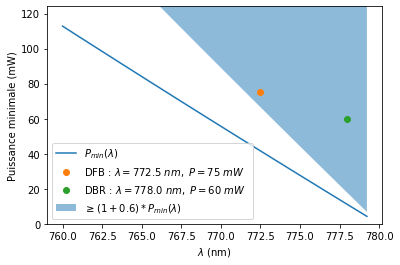
\includegraphics[width=0.7\linewidth]{Dipolaire/Figures/Power_min_lambda}
    \caption{La ligne pleine représente $P_{\text{min}}(\lambda)$ et le fond bleu représente $(1 + 60\% ) P_{\text{min}}(\lambda)$}
\end{figure}

{\color{gray} \tiny  
	\item Dans le commerce on trouve des laser avec une longueur d'onde $\lambda = 765~nm$. On note $\omega \equiv 2 \pi c / \lambda $. $P_{\text{min}} = 85.0~\text{mW}$ 

$$
\begin{array}{rl}
	\mbox{Ref} & \mbox{\tiny EYP-TPA-0765-01500-3006-CMT03-0000/ EYP-TPA-0765-01500-3006-BTU02-0000}\\
	\mbox{Wavelength} & 	765 ~nm\\
	\mbox{Power} & 1,5~ W\\
	\mbox{Laser Type} & \mbox{Tapered Amplifier}\\
	\mbox{Operation Mode} & CW\\
	\mbox{Quote} & ? / ?
\end{array}
$$
\url{https://www.toptica-eagleyard.com/ey-product/eyp-tpa-0765-01500-3006-cmt03-0000/?_application%5B0%5D=quantum-technology&_application[]=spectroscopy}\\
\url{https://www.toptica-eagleyard.com/ey-product/eyp-tpa-0765-01500-3006-btu02-0000/?_application%5B0%5D=quantum-technology&_application[]=spectroscopy}

	\item $\lambda = 770~nm$ . $P_{\text{min}} = 55.6~\text{mW}$
$$
\begin{array}{rl}
	\mbox{Ref} & \mbox{EYP-ECL-0770-00080-1500-BFW01-0005}\\
	\mbox{Wavelength} & 	770 ~nm\\
	\mbox{Power} & 80 ~ mW\\
	\mbox{Laser Type} & \mbox{ECL laser diode}\\
	\mbox{Operation Mode} & CW\\
	\mbox{Quote} & ?
\end{array}
$$ 
\url{https://www.toptica-eagleyard.com/ey-product/eyp-ecl-0770-00080-1500-bfw01-0005/?_application%5B0%5D=atomic-clock&_application%5B1%5D=cold-atom-interferometry&_application%5B2%5D=metrology&_application[]=quantum-technology}	

}
\end{itemize}

}
